%------------------------------------------------
% Quick reference. 
%------------------------------------------------
%
% Для вставки картинок:
%
%--------         Комманда
%
%\begin{figure}[H]
%	\includegraphics{img_name}
%	\caption{some caption}
%	\label{some_pic}
%\end{figure}
%
%--------        Переменные
%
% img_name     <- Название картинки в папке img.
% some_caption <- подпись картинки.
% label        <- лейбл нужен для ссылок на картинку.
% H            <- расположение картинки на странице.
% Чтобы сентрировать добавьте параметр \centering перед строчкой \includegraphics{}
% Чтобы вместить большой рисунок добавьте [width=\textwidth,height=\textheight,keepaspectratio] как параметр к \includegraphics{}
%--------         Пример
%
%\begin{figure}[H]
%   \centering
%	\includegraphics[width=\textwidth,height=\textheight,keepaspectratio]{pic1.jpg}
%	\caption{График зависимости какой-то хуйни}
%	\label{grapics1}
%\end{figure}
%
%------------------------------------------------
%
% Для референса по лейблу:
%
%--------         Комманда
%
% Для ссылки используется \eqref{ref}.
%
%--------        Переменные
%
% ref          <- указанный лейбл в директиве \label{ref}
%                 Ссылку можно сделать на любой объект имеющий \label{•}
%
%--------         Пример
%
% \eqref{graphics1}
%
%------------------------------------------------
%
% Для листинга кода:
%
%--------         Комманда
%
% \lstinputlisting[language=lang,mathescape=true]{src}
%--------        Переменные
%
% lang         <- язык на котором написан исходный код, например "python" или "C++".
% mathescape   <- если в исходниках есть формулы LaTeX, то они будут представлены как формулы.
% src          <- путь до файла исходников.
%
%--------         Пример
%
% \lstinputlisting[language=C++,mathescape=false]{./src/bullshit.cpp}
%
%------------------------------------------------
%
% Для вставки таблиц:
%
%--------
%\begin{table}[H]
%	\centering
%	\caption{ capt }
%	\begin{tabularx}{0.9\textwidth}{ | Y | Y | }
%		\hline
%		lines
%	\end{tabularx}
%	\label{tab1}
%\end{table}
%--------
% caption      <- Подпись таблицы.
% tab1         <- лейбл нужный для ссылки на таблицу.
% | Y | Y |    <- количество и формат столбцов.
% Y            <- Тип столбца.
%                 В данном случае определены кастомные столбцы Y (Спасибо Максиму Наумову)
% |            <- обозначает границы столбца.
%                 То есть, если будет указано |Y Y|, то столбцы внутри строк разделены не будут.
% H            <- То же самое, что и у картинок.
% lines        <- непосредственно элементы таблицы.
%                 Разделяются знаком "&", оканчивать каждую строку лучше \\ \hline
%
%--------         Пример
%\begin{table}[H]
%	\centering
%	\caption{ capt }
%	\begin{tabularx}{0.9\textwidth}{ | Y | Y | }
%		\hline
%		str1 & str2 \\ \hline
%		str1 & str2 \\ \hline
%		str1 & str2 \\ \hline
%		str1 & str2 \\ \hline
%		str1 & str2 \\ \hline
%	\end{tabularx}
%	\label{tab1}
%\end{table}
%------------------------------------------------

\documentclass[12pt, fleqn]{article}

\makeatletter
\renewcommand*\l@section{\@dottedtocline{1}{1.5em}{2.3em}}



%\includegraphics{universe}

\usepackage[utf8]{inputenc}
\usepackage[T2A]{fontenc}
\usepackage[russian]{babel} % указывает язык документа
\usepackage[left=3cm,right=2cm,top=2cm,bottom=2cm,bindingoffset=0cm]{geometry}
\usepackage{lastpage}
\usepackage{fancyhdr}
\usepackage{titlesec}
\usepackage{graphicx} % для вставки картинок
\usepackage[intlimits]{mathtools} % математические дополнения
\usepackage{amssymb}
\usepackage[tableposition=top]{caption}
\usepackage{subcaption}
\usepackage{indentfirst}
\usepackage{pythonhighlight}
\usepackage{listings}
\usepackage{tabularx}
\usepackage{tabulary}
\usepackage{multirow}
\usepackage{float}
\usepackage[figure,table]{totalcount}
\usepackage{diagbox}
\usepackage[german=guillemets]{csquotes}
\usepackage{fontspec} 
\usepackage{enumitem}
%\usepackege{xparse}
%\usepackage{mathptmx}% http://ctan.org/pkg/mathptmx
%\usepackage{showframe}
\usepackage{hyperref}

\setlength{\parindent}{1.2cm}

\setlength{\mathindent}{1.2cm}

\defaultfontfeatures{Ligatures={TeX},Renderer=Basic} 
\setmainfont[Ligatures={TeX,Historic}]{Times New Roman}

%\setlist[enumerate]{itemindent=\dimexpr\labelwidth+\labelsep\relax,leftmargin=0pt}

%\setlength{\section*}{0.5cm}
%\usepackage{minted}
%\usepackage{fancyvrb}
%\usepackage{newtxtext}

%\titleformat{\section}[hang]{\bfseries\LARGE\centering}{}{1em}{}

%\setlist[enumerate]{itemindent=\dimexpr\labelwidth+\labelsep\relax,leftmargin=0pt}
\setlist[enumerate,itemize]{leftmargin=0pt,itemindent=1.7cm}
\titleformat{\section}{\large\bfseries\centering}{\thesection}{0.5em}{\MakeUppercase}
\titleformat{\subsection}[block]{\bfseries\hspace{1em}}{\thesubsection}{0.5em}{}
%\setlength{\subsection*}{1.5cm}
%\setlength{\parindent}{4em}

%\setlength{\parindent}{1.5cm}

\captionsetup[figure]{labelfont={it},textfont={it},name={Рисунок},labelsep=endash, skip=5pt}
\captionsetup[table]{labelfont={it},textfont={it},name={Таблица},labelsep=endash,singlelinecheck=false, skip=5pt, margin=1cm}


%\renewcommand{\baselinestretch}{1.5}
\linespread{1.5} % полуторный интервал
\frenchspacing
\graphicspath{ {images/} }

  %-------------------------------------------
  % Переменные
  %-------------------------------------------

  \newcommand{\firstAuthorSurName}{Белоусов} 					                           % Фамилия автора.
  \newcommand{\firstAuthorInitials}{ А. А. } 					                           % Фамилия автора.
  \newcommand{\leftcolon}{Уравнения Математической Физики}
  \newcommand{\secondAuthorSurName}{Посоха} 					                           % Фамилия автора.
  \newcommand{\secondAuthorInitials}{ К. А.} 					                           % Фамилия автора.
  \newcommand{\teacherName}{Дегтярев А. А.}				                               % Имя преподавателя.
  \newcommand{\variantNumber}{40} 							                           % Номер варианта.
  \newcommand{\groupNumber}{6409-010302D} 				                               % Номер группы.
  \newcommand{\subjectTitle}{Отчет по курсовой работе}                                  % Название предмета.
  \newcommand{\taskTitle}{Дисциплина \enquote{Уравнения математической физики}} 		  % Название работы.
  \newcommand{\theme}{АНАЛИТИЧЕСКОЕ РЕШЕНИЕ КРАЕВЫХ ЗАДАЧ МАТЕМАТИЧЕСКОЙ ФИЗИКИ} 		  % Название работы.
  
  %-------------------------------------------
  % Ссылки в оглавлении
  %-------------------------------------------
  

\hypersetup{
    colorlinks,
    citecolor=black,
    filecolor=black,
    linkcolor=black,
    urlcolor=black
}

  %-------------------------------------------
  % Стиль футеров и хедеров
  %-------------------------------------------

\pagestyle{fancy}
\fancyhead[L, R]{}
\fancyfoot[L]{}
\fancyfoot[R]{}
\renewcommand{\footrulewidth}{0pt}
\renewcommand{\headrulewidth}{0pt}

%\renewcommand\subsectionfont{\normalfont\normalsize\bfseries}

\def\l@subsection{\@dottedtocline{2}{3.8em}{3.2em}}

% Для листинга

\lstset{
basicstyle=\footnotesize\ttfamily,
columns=fullflexible,
keywordstyle=\color{blue},
%frame=single,
breaklines=true,
numberstyle=\tiny\color{mygray},
postbreak=\mbox{\textcolor{red}{$\hookrightarrow$}\space},
showstringspaces=false,
}

\newcolumntype{Y}{>{\centering\arraybackslash}X}
\renewcommand{\tabularxcolumn}[1]{m{#1}} % Для вертикального центрировая табличных ячеек.

\begin{document}

%----------------------------------------------------------------------------------------
%	TITLE PAGE
%----------------------------------------------------------------------------------------
\pagenumbering{Alph}

\begin{titlepage}
							
	\center
							
	%------------------------------------------------
	%	Заголовки
	%------------------------------------------------
							
	\textsc{Министерство образования и науки Российской Федерации}\\[-0.15cm]
	\textsc{Федеральное государственное автономное образовательное учреждение \\[-0.15cm] высшего образования}\\[-0.15cm] 
	\textsc{«Самарский национальный исследовательский университет \\[-0.15cm] имени академика С.П.Королёва»}\\[0.25cm]
	\textsc{Факультет информатики}\\[0.1cm]
	\textsc{Кафедра технической кибернетики}\\[0.5cm]
						
	%------------------------------------------------
	%	Название работы
	%------------------------------------------------
							
	\vfill\vfill
						    
							
	{\large \textbf{\subjectTitle}}\\[0.3cm]
	
	{\large \taskTitle}\\[0.5cm]
						  
    {\large Тема: \enquote{\textbf{\theme}}}\\[0.5cm]

    \vfill
    
   {Вариант № \variantNumber}\\[0.5cm]


	\vfill\vfill
							
	\begin{minipage}{1\textwidth}
		\begin{center}
			\begin{tabularx}{\textwidth}{X l}
				Выполнил студент:        & \firstAuthorSurName \firstAuthorInitials \\
				Группа:                    & 6409                     		           \\
				Проверил:                  & \teacherName         		                \\
			\end{tabularx}
		\end{center}
	\end{minipage}
							
						
	%------------------------------------------------
	%	Дата
	%------------------------------------------------
							
	\vfill\vfill\vfill
					
	{\centering Самара \the\year}
							
							
\end{titlepage}

\pagenumbering{arabic}

\setcounter{page}{2}


%------------------------------------------------
%Задание
%------------------------------------------------

\section*{Задание к курсовой работе}
{
	\begin{enumerate}
	    \item Осуществить  математическую  постановку  краевой  задачи  для физического процесса, описанного в предложенном варианте курсовой работы.
        \item Используя  метод  разделения  переменных  (метод  Фурье),  получить решение краевой задачи в виде разложения в ряд Фурье по собственным функциям оператора Лапласа, соответствующим краевым условиям задачи.
        \item Провести анализ погрешности решения.
        \item Разработать  компьютерную  программу  расчета  функции-решения краевой  задачи  (суммирования  ряда  Фурье). При  расчете коэффициентов ряда использовать метод численного интегрирования, если  это  необходимо. Если необходимо, то разработать специальный программный модуль для вычисления используемых собственных чисел оператора Лапласа. Компьютерная  программа  должна  обеспечивать  возможность  диалогового режима  ввода  физических,  геометрических параметров  задачи,  числа суммируемых  элементов  ряда,  графическую  визуализацию  рассчитанного решения задачи.
        \item Оформить отчет о выполненной курсовой работе.
	\end{enumerate}
}
\newpage

\section*{\underline{\textit{Вариант} 40}}{
    Разработать программу расчета на промежутке времени $0<t \le T$ малых поперечных колебаний прямоугольной однородной мембраны шириной $l_x$ и длиной $l_y$. Колебания мембраны возбуждаются начальным отклонением
    $$u(x,y,t=0)=\alpha(x,y), 0 \le x \le l_x, 0 \le y \le l_y. $$ 
   
    Края мембраны $x=0, x=l_x, y=0$ и $y=l_y$ жестко закреплены, а реакция окружающей среды пренебрежимо мала. Начальные скорости точек мембраны равны нулю.
    
    Поверхностная плотность мембраны и величина натяжения, возникающего в ней в процессе колебаний, равны $\rho$ и $\eta$ соответственно.
   
    Для решения описанной задачи математической физики применить метод разделения переменных. Для расчетов использовать представление решения задачи в виде ряда Фурье по собственным функциям оператора Лапласа, удовлетворяющим соответствующим краевым условиям.
    
    При проведении расчетов использовать значения параметров $l_x, l_y, T, \rho, \eta,$ а также выражение функции $\alpha(x,y),$ указанные преподавателем.
    
    Значения параметров, указанные преподавателем:
    
    %{\renewcommand{\arraystretch}{1.6}%
    \bgroup
    \def\arraystretch{1.6}%  1 is the default, change whatever you need
    \begin{tabular}{rcl}
    $l_x$ & = & $4,$ \\ 
    $l_y$ & = & $1,$ \\
    $T$ & = & $10,$ \\
    $\rho$ & = & $1,$ \\
    $\eta$ & = & $1,$ \\
    $\alpha(x, y)$ & = & $ p(x,y)\sin(\dfrac{\pi y}{l_y}) $ \\
    $p(x,y)$ & = & $ \dfrac{x^2}{4} + x \quad $ \\

    \end{tabular} 
    \egroup

}

\newpage
\section*{РЕФЕРАТ}{
	\begin{center}
	\pageref{LastPage} страниц,
	\totalfigures\ рисунков,
	\totaltables\ таблиц,
	0 источников,
	1 приложение
	\end{center}
	
    \begin{center}
       УРАВНЕНИЯ МАТЕМАТИЧЕСКОЙ ФИЗИКИ, КРАЕВАЯ  ЗАДАЧА, УРАВНЕНИЕ ТЕПЛОПРОВОДНОСТИ,
        МЕТОД РАЗДЕЛЕНИЯ ПЕРЕМЕННЫХ, СОБСТВЕННЫЕ ФУНКЦИИ ОПЕРАТОРА ЛАПЛАСА, РЯД 
        ФУРЬЕ, ПОЛИНОМ ЛЕЖАНДРА.     
    \end{center}
    

Целью курсовой работы является получение решения краевой задачи колебаний прямоугольной мембраны в виде разложения в ряд Фурье по собственным функциям оператора Лапласа и создание компьютерной программы для расчета функции-решения.

Для  получения  аналитического  решения  краевой  задачи  использован 
метод разделения переменных. Решение задачи получено в виде конечного ряда Фурье.

Разработана  компьютерная  программа,  обеспечивающая  расчет  и 
графическую  визуализацию  процесса колебаний мембраны.

Приведены  графические  результаты  численного  решения  задачи колебаний мембраны, а также анализ погрешности решения.

Программа  написана  на  языке Python в  среде  разработки PyCharm на операционной системе Windows. 

}

\newpage
\tableofcontents
\newpage
\phantomsection
\addcontentsline{toc}{section}{Введение}
%------------------------------------------------
%Введение
%------------------------------------------------

\section*{Введение}
{
Метод разделения переменных относится к классу аналитических
методов решения краевых задач математической физики. Характеризуя этот
метод необходимо выделить его достоинства и недостатки в сравнении с
другими методами.

К достоинствам метода разделения переменных следует отнести
возможность получения точного решения краевой задачи в виде ряда Фурье.
Такая форма решения задачи часто и весьма успешно используется для
теоретического исследования свойств этого решения. В случае достаточно
быстрой сходимости ряда Фурье она может с успехом использоваться для
численного моделирования физического процесса (явления).

К числу недостатков метода следует отнести его невысокую
универсальность. Этот метод весьма проблематично использовать для
решения нелинейных уравнений математической физики, уравнений с
переменными операторными коэффициентами, а также для решения краевых
задач в областях со сложными границами.

Суть метода разделения переменных состоит в факторизации по
каждой независимой переменной функции, определяющей решение
уравнения математической физики. Далее осуществляется переход к так
называемой задаче Штурма-Лиувилля, решение которой приводит к
получению собственных функций и соответствующих им собственных чисел
оператора Лапласа. Затем решение исходной задачи ищется в виде ряда
Фурье по этим собственным функциям.
    
В настоящей работе метод разделения переменных применен для
получения аналитической формы решения задачи описания процесса колебаний мембраны.
На основе этого результата разработан алгоритм и компьютерная программа
численного моделирования процесса колебаний мембраны.    
}
\newpage

%------------------------------------------------
% Начало основной части
%------------------------------------------------
\titleformat{\section}{\large\bfseries}{\thesection}{0.5em}{}
\titlespacing*{\section}{\parindent}{1ex}{1em}
\section{Постановка краевой задачи}
{

Построим математическую модель поперечных колебаний тонкой однородной мембраны.
Уравнение свободных поперечных колебаний мембраны имеет вид:
    \begin{equation}\label{source_func}
      \dfrac{\partial u}{\partial t} = \alpha^2(
      \dfrac{\partial u}{\partial x} + 
      \dfrac{\partial u}{\partial y}).
    \end{equation}

В условии задачи указано, что края мембраны жестко закреплены. Отсюда
    следуют граничные условия:
    \begin{equation}
    u|_{x=0}, 
    u|_{y=0},  
    u|_{x=l_x}, 
    u|_{y=l_y} = 0.
    \end{equation}
    
По условию, в начальный момент времени отклонение мембраны задано функцией $\alpha(x, y)$, а начальная скорость точек мембраны равна нулю. Отсюда получаем начальные условия:
    \begin{align*}
        &  u|_{t=0} = p(x,y)\sin(\dfrac{\pi y}{l_y});\\        
        & \dfrac{\partial u}{\partial t}|_{t=0} = 0.
    \end{align*}
    
Производим следующую замену:
     \begin{equation}\label{change}
    	u(x,y,t) = \nu(x,t)\sin (\dfrac{\pi y}{l_y}).
    \end{equation}    
    
Подставляем в исходное уравнение, переходим к виду:
    \begin{equation}
         \dfrac{\partial \nu}{\partial t} = \alpha^2(\dfrac{\partial \nu}{\partial x}
        - \dfrac{\pi^2}{l_y}\nu(x, t)).
    \end{equation}
    
    Пересчитываем начальные условия для $\nu(x,y)$:
     \begin{align*}
        &  \nu|_{t=0} = p(x,y);\\        
        & \dfrac{\partial \nu}{\partial t}|_{t=0} = 0.
    \end{align*}
    
    
   Таким образом, имея уравнение, набор граничных и начальных условий, получим математическую модель, описывающую нашу задачу:
   		\begin{equation}
   		    \dfrac{\partial u}{\partial t} = \nu(x,t)\sin (\dfrac{\pi y}{l_y});
   		\end{equation}
        \begin{equation}\label{eq15}
            \left\{
			\begin{split}
			& \dfrac{\partial \nu}{\partial t} = \alpha^2(\dfrac{\partial \nu}{\partial x}
        - \dfrac{\pi^2}{l_y}\nu(x, t)), 0 \le x \le \l_x; \\
			 &\nu|_{x=0},   
    \nu|_{x=l_x} = 0;\\
            &  \nu|_{t=0} = p(x,y);\\        
        	& \dfrac{\partial \nu}{\partial t}|_{t=0} = 0;
			\end{split}
			\right.
        \end{equation}
}
\newpage
\section{Аналитическое решение  краевой  задачи  и  получение  решения задачи в виде ряда Фурье}
{

Для решения поставленной задачи в уравнении \eqref{eq15} воспользуемся методом разделения переменных:
    \begin{equation}\label{eq16}
        \nu(x,t) = X(x)T(t).
    \end{equation}

Тогда уравнение \eqref{eq15} примет вид:    
    \begin{align*}
        &T''X = \alpha^2 \left(X''T - \dfrac{\pi^2}{l_y^2} XT \right);        
    \end{align*}
Разделим обе части на $a^2XT$ и получим следующее уравнение:
    \begin{equation}\label{eq17}
        \dfrac{T'}{\alpha^2T} = \dfrac{X''-\dfrac{\pi^2}{l_y^2}X}{X}.
    \end{equation}

В равенстве \eqref{eq17} можно заметить, что левая и правая части зависят только от $t$ и  $\theta$ соответственно. Тем самым, общая величина выражений - константа, которую мы возьмем равной $-\lambda^2$. Константа берется с отрицательным знаком, чтобы удовлетворять граничным условиям. Таким образом равенство \eqref{eq17} примет вид:

\begin{equation}\label{eq17}
        \dfrac{T'}{\alpha^2T} = \dfrac{
        X''-\dfrac{\pi^2}{l_y^2}X}{X} = -\lambda^2.
\end{equation}

Откуда получим два уравнения:
\begin{align*}
		& T''+\lambda^2\alpha^2T=0;\\
		& X''+(\lambda^2-\dfrac{\pi^2}{l_y^2})X = 0.
\end{align*}

%%========================================================================



И обозначим, что в силу начальных условий, $z \in [-1; 1]$. После подстановки $\omega$ из уравнения \eqref{eq16} будет зависеть от $z$ и $t$. 
Выразим производные от $X$ по $\theta$ через производные от $X$ по $z$. 

\begin{align*}
    &\dfrac{\partial X}{\partial z} = \dfrac{\partial X}{\partial \theta}  \dfrac{\partial \theta}{\partial z}; \\
    &\dfrac{\partial X}{\partial \theta} = - \text{sin}(\theta) \dfrac{\partial X}{\partial z}; \\
    &\dfrac{\partial^2 X}{\partial \theta^2} = (1 - z^2)\dfrac{\partial^2 X}{\partial z^2} - z\dfrac{\partial X}{\partial z}.
\end{align*}

Тогда уравнение \eqref{eq19} примет вид:
    \begin{equation}\label{eq20}
    (1-z^2)\dfrac{\partial^2 X}{\partial x^2} - 2z\dfrac{\partial X}{\partial z} +  X (\dfrac{-\alpha}{kl} + \dfrac{\lambda}{k}) = 0.
    \end{equation}
    
    Произведем замену переменных в уравнении \eqref{eq20}.
    Пусть: 
    \begin{equation}\label{for_lambda}
        (\dfrac{-\alpha}{kl} + \dfrac{\lambda}{k}) = n(n+1).
    \end{equation}
    Тогда:
    \begin{equation}\label{eq21}
    (1-z^2)\dfrac{\partial^2 X}{\partial x^2} - 2z\dfrac{\partial X}{\partial z} +  n(n+1)X = 0.
    \end{equation}
    
    Нетрудно заметить, что уравнение \eqref{eq21} является уравнением Лежандра, описанное в приложении А, решением которого являются полиномы Лежандра.
    
    Функция Лежандра образует базис в некотором пространстве. Разложим функцию $\omega(z,t)$ в ряд, взяв за базис $P_n(z)$, и  пусть $X_n(z) = P_n(z)$. Тогда будем искать решение в виде:
    \begin{equation}\label{eq24}
    \omega(z,t) = \sum_{n=0}^{\infty}{\hat{A_n} P_n(z) T_n(t)}.
    \end{equation}
    

    Тогда для нахождения $\omega(z, t)$ из уравнения \eqref{eq24} требуется вычислить $T_n(t)$. Для этого из левой части уравнения \eqref{eq18} выразим $T_n$.
    
    \begin{align*}
        &c\dfrac{T'}{T} = -\lambda;  \\
        &\dfrac{d T}{T d t} = \dfrac{- \lambda}{c};\\
        &\int\limits{\dfrac{d T}{T}} = \int\limits{\dfrac{- \lambda dt}{c}}; \\
    \end{align*}
    
    \begin{equation}\label{eq25}
        T_n = C_n e^{\dfrac{-\lambda_n t}{c}},
    \end{equation}        
    где $C_n$ - константа для $n$-го члена.
    
        Тогда из формулы \eqref{for_lambda} видно, что $\lambda_n$, необходимая для вычисления $T_n$, будет находится следующим образом:
    \begin{equation}\label{eq26}
        \lambda_n = k(n^2 + n + \dfrac{\alpha}{kl}).
    \end{equation}
    
    Следовательно, уравнение \eqref{eq24} примет вид:
    
    \begin{equation}\label{eq27}
        \omega(z,t) = \sum_{n=0}^{\infty}{A_n P_n(z) e^{\dfrac{-k(n^2 + n + \dfrac{\alpha}{kl}) t}{c}}},
    \end{equation}
    где $A_n = \hat{A_n} \cdot C_n$.
    
    Воспользуемся начальным условием и зафиксируем $t$ в момент времени $t=0$ и получим:
    \begin{equation}\label{eq28}
       \omega(z,t)|_{t=0} = \sum_{n=0}^{\infty}{A_n P_n(z)} = \psi(z) - u_c
    \end{equation}
    
    Следует указать два важных свойства полиномов Лежандра:
    
    \begin{equation}\label{sv_pol1}
        \int\limits_{-1}^{1}{P_n(x)P_m(x)dx = 0, \text{ при } m \ne n};
    \end{equation}
    
    \begin{equation}\label{sv_pol2}
        \int\limits_{-1}^{1}{\left[ P_n(x) \right]^2} = \dfrac{2}{2n+1}
    \end{equation}
    
    Поэтому домножим функцию \eqref{eq28} на полином Лежандра порядка $m$ и проинтегрируем по $z$, чтобы можно было применить свойство описанное в равенстве \eqref{sv_pol1}.
    
    \begin{align*}
       &\omega(z)|_{t=0} = \sum_{n=0}^{\infty}{A_n P_n(z)} \bigg| \cdot P_m(z); \\
       &(\psi(z) - u_c) P_m(z) = \sum_{n=0}^{\infty}{A_n P_n(z) P_m(z)};  \\
       &\int\limits_{-1}^{1}{(\psi(z) - u_c) P_m(z) dz} = \int\limits_{-1}^{1}{\sum_{n=0}^{\infty}{A_n P_n(z) P_m(z)} dz}; \\
       &\text{В силу свойства \eqref{sv_pol1}: } \\
       &\int\limits_{-1}^{1}{(\psi(z) - u_c) P_m(z) dz} = A_m \int\limits_{-1}^{1}{{P_m^2(z)} dz}; \\
       &A_m = \dfrac{\int\limits_{-1}^{1}{(\psi(z) - u_c) P_m(z) dz}}{\int\limits_{-1}^{1}{{P_m^2(z)} dz}}.
    \end{align*}
    Воспользуемся формулой \eqref{sv_pol2} для нахождения знаменателя $A_m$ и получим:
    \begin{align}\label{A_n}
        A_m =  \dfrac{(2m + 1) \int\limits_{-1}^{1}{(\psi(z) - u_c) P_m(z) dz}}{2}.
    \end{align}
     
    Таким образом было получено аналитическое решение поставленной задачи. Конечная формула ряда будет выглядеть следующим образом:
    
    \begin{equation}\label{final_series}
        \omega(z,t) = \dfrac{1}{2} \sum_{n=0}^{\infty}{(2n + 1) e^{\dfrac{-k(n^2 + n + \dfrac{\alpha}{kl}) t}{c}}  P_n(z) \int\limits_{-1}^{1}{\left[(\psi(z) - u_c) P_n(z)\right]dz}}.
    \end{equation}
}

\newpage
\section{Получение расчетной формулы для начальной функции  \texorpdfstring{$\psi_1$}{TEXT} (Кирилин П. Н.)}
{

Преподавателем была выдана функция, задающая начальное условие:
    \begin{equation}
        \psi(\theta) = u_c + \text{cos}^4\theta.     
    \end{equation}
    
    С учетом замены переменной, которая была произведена ранее ($z = cos(\theta)$), функция $\psi(z)$ будет иметь вид: 
    \begin{align*}
        \psi(z) = u_c + z^4.
    \end{align*}
    
    Подставляя полученные данные в формулу \eqref{eq28}, получим:    
    \begin{equation}
      \omega(z,t)|_{t=0} = \sum_{n=0}^{\infty}{A_n P_n(z)} = z^4.
    \end{equation}
    
    В следствии начального условия можно утверждать, что ряд конечен 
    и полиномы Лежандра, включенные в ряд, не превышают 4-ого порядка.
    Тогда $\omega(z, t)|_{t=0}$ примет вид:
    % \dfrac{(2m + 1) \int\limits_{-1}^{1}{z^4 P_m(z) dz}}{2}
    \begin{align}
        \omega(z, t)|_{t=0} =  A_0 + A_1 z + A_2 \frac{1}{2}(3z^2-1) + A_3 \frac{1}{2}(5z^3-3z) + A_4 \frac{1}{8}(35z^4-30z^2+3).
    \end{align}
    Раскрыв скобки и приведя подобные слагаемые, получим:
    \begin{align}\label{eq34}
        A_0 - \frac{1}{2}A_2 + \frac{3}{8}A_4 + z(A_1 - \frac{3}{2}A_3) + z^2(\frac{3}{2}A_2 - \frac{30}{8}A_4) +
        \frac{5}{2}A_3 z^3 + \frac{35}{8} A_4 z^4 = z^4
    \end{align}
    Решим \eqref{eq34}. Для этого составим следующую систему:
    \begin{equation}\label{eq35}
    \left\{
    \begin{split}
     &A_0 - \frac{1}{2}A_2 + \frac{3}{8}A_4  = 0, \\
     &A_1 - \frac{3}{2}A_3 = 0, \\
     &\frac{3}{2}A_2 - \frac{30}{8}A_4 = 0, \\
     &\frac{5}{2}A_3 = 0, \\
     &\frac{35}{8} A_4 = 1.
    \end{split}
    \right.
    \end{equation} 
    
    Система \eqref{eq35} решается однозначно, и решение выглядит следующим образом:
    
    \begin{equation}
    \left\{
    \begin{split}
     &A_0 = \frac{1}{5}, \\
     &A_1 = 0, \\
     &A_2 = \frac{4}{7}, \\
     &A_3 = 0, \\
     &A_4 = \frac{8}{35}.
    \end{split}
    \right.
    \end{equation} 
    
    Подставив полученные значения $A_n$ в  получим:
    \begin{equation}
        \omega(z,t) = \frac{1}{5}e^{- \dfrac{\lambda_0 t}{c}} + \frac{4}{14}(3z^2-1)e^{- \dfrac{\lambda_2 t}{c}} + 
        \frac{1}{35}(35z^4-30z^2+3)e^{- \dfrac{\lambda_4 t}{c}},
    \end{equation}
    где $\lambda_n$ вычисляется по формуле \eqref{eq26}.
    
%    Была получена расчетная формула для начальной функции $\psi_1(z),\text{где } z = cos(\theta), z \in [-1, 1].$
    Совершим обратные замены \eqref{replacement_omega} и \eqref{replacement_z} для получения конечной формулы, удовлетворяющей поставленной задаче:
    \begin{align*}
       &\omega(\theta,t) =  
        \frac{1}{5}e^{- \dfrac{\lambda_0 t}{c}} + \frac{4}{14}(3\text{cos}^2(\theta)-1)e^{- \dfrac{\lambda_2 t}{c}} + 
        \frac{1}{35}(35\text{cos}^4(\theta)-30\text{cos}^2(\theta)+3)e^{- \dfrac{\lambda_4 t}{c}};
    \end{align*}
    \begin{align}\label{series_kirilin}
    \upsilon(\theta, t) = \omega(\theta, t) + u_c = 
         &\frac{1}{5}e^{- \dfrac{\lambda_0 t}{c}} + \frac{4}{14}(3\text{cos}^2(\theta)-1)e^{- \dfrac{\lambda_2 t}{c}} 
        + \frac{1}{35}(35\text{cos}^4(\theta) - \nonumber\\
        &-30\text{cos}^2(\theta)+3)e^{- \dfrac{\lambda_4 t}{c}} + u_c.
    \end{align}
    Из-за конечного количества элементов в ряде \eqref{series_kirilin} остаток ряда отсутствует.


\newpage
\section{Получение расчетной формулы для начальной функции \texorpdfstring{$\psi_2$}{TEXT} (Посоха К.А.)}
{
Преподавателем была выдана функция, задающая начальное условие:
    \begin{equation}
        \psi(\theta) = u_c + \text{cos}^5\theta.     
    \end{equation}
    
     После проведенной замены переменной, которая была произведена ранее ($z = cos(\theta)$), функция $\psi(z)$ примет вид: 
    \begin{align*}
        \psi(z) = u_c + z^5.
    \end{align*}
    
    Подставляя полученные данные в формулу \eqref{eq28}, получим:    
    \begin{equation}
      \omega(z,t)|_{t=0} = \sum_{n=0}^{\infty}{A_n P_n(z)} = z^5.
    \end{equation}
    
    	 Из-за начального условия можно полагать, что ряд является конченым, состоящий из 6 слагаемых, 
а полиномы Лежандра, включенные в ряд, не будут превышать 5-ого порядка.
    Тогда $\omega(z, t)|_{t=0}$ примет вид:
    % \dfrac{(2m + 1) \int\limits_{-1}^{1}{z^4 P_m(z) dz}}{2}
    \begin{align}
        &\omega(z, t)|_{t=0} =  A_0 + A_1 z + A_2 \frac{1}{2}(3z^2-1) + A_3 \frac{1}{2}(5z^3-3z) 
        + A_4 \frac{1}{8}(35z^4-30z^2+3) + \nonumber\\
         &  +  A_5 \frac{1}{8}(63z^5-70z^3+15z).
    \end{align}
    %$  +  A_5 \dfrac{1}{8}(63z^5-70z^3+15z).$
    
    
    
    Раскрыв скобки и приведя подобные слагаемые, получим:
    \begin{align}\label{eq43}
        &A_0 - \frac{1}{2}A_2 + \frac{3}{8}A_4 + z(A_1 - \frac{3}{2}A_3 + \frac{15}{8}A_5) + z^2(\frac{3}{2}A_2 - \frac{30}{8}A_4) +
        z^3 ( \frac{5}{2}A_3 - \frac{70}{8}A_5) + \nonumber\\
          &+ \frac{35}{8} A_4 z^4 + \frac{63}{8} A_5 z^5 = z^5
    \end{align}
    
    Решим \eqref{eq43}. Для этого составим следующую систему:
    \begin{equation}\label{eq44}
    \left\{
    \begin{split}
     &A_0 - \frac{1}{2}A_2 + \frac{3}{8}A_4  = 0, \\
     &A_1 - \frac{3}{2}A_3 + \frac{15}{8}A_5 = 0, \\
     &\frac{3}{2}A_2 - \frac{30}{8}A_4 = 0, \\
     & \frac{5}{2}A_3 - \frac{70}{8}A_5 = 0, \\
     &\frac{35}{8} A_4 = 0, \\
     &\frac{63}{8} A_5 = 1.
    \end{split}
    \right.
    \end{equation} 
    
    Система \eqref{eq44} решается однозначно, и решение выглядит следующим образом:
    
    \begin{equation}
    \left\{
    \begin{split}
     &A_0 = 0, \\
     &A_1 = \frac{27}{63}, \\
     &A_2 = 0, \\
     &A_3 = \frac{28}{63}, \\
     &A_4 = 0, \\
     &A_5 = \frac{8}{63}
    \end{split}
    \right.
    \end{equation} 
    
    Подставив полученные значения $A_n$ в  получим:
    % e^{- \dfrac{\lambda_n t}{c}}
    \begin{equation}
        \omega(z,t) = \frac{27}{63}ze^{- \dfrac{\lambda_1 t}{c}} + \frac{14}{63}(5z^3-3z)e^{- \dfrac{\lambda_3 t}{c}} + 
        \frac{1}{63}(63z^5-70z^3+15z)e^{- \dfrac{\lambda_5 t}{c}},
    \end{equation}
    где $\lambda_n$ вычисляется по формуле \eqref{eq26}.
    
        %Была получена расчетная формула для начальной функции $\psi_1(z),\text{где } z = cos(\theta), z \in [-1, 1].$
        
        Совершим обратные замены \eqref{replacement_omega} и \eqref{replacement_z} для получения конечной формулы, удовлетворяющей поставленной задаче:
        
        \begin{align*}
       &\omega(\theta,t) = \frac{27}{63}\text{cos}(\theta)e^{- \dfrac{\lambda_1 t}{c}} + \frac{14}{63}(5\text{cos}^3(\theta)-3\text{cos}(\theta))e^{- \dfrac{\lambda_3 t}{c}} + \\
         &+ \frac{1}{63}(63\text{cos}^5(\theta)-70\text{cos}^3(\theta)+15\text{cos}(\theta))e^{- \dfrac{\lambda_5 t}{c}};
    \end{align*}
    
    \begin{align}\label{series_posoha}
    &\upsilon(\theta, t) = \omega(\theta, t) + u_c = 
         \frac{27}{63}\text{cos}(\theta)e^{- \dfrac{\lambda_1 t}{c}} + \frac{14}{63}(5\text{cos}^3(\theta)-3\text{cos}			(\theta))e^{- \dfrac{\lambda_3 t}{c}} + \nonumber\\
        & + \frac{1}{63}(63\text{cos}^5(\theta)-70\text{cos}^3(\theta)+15\text{cos}(\theta))e^{- \dfrac{\lambda_5 t}{c}} 			+ u_c.
    \end{align}
    
        
    Из-за конечного количества элементов в ряде \eqref{series_posoha} остаток ряда отсутствует.    
    
   
}


\newpage
\section{Анализ погрешности решения и вычислительной сложности алгоритма}{ 
 При помощи формулы \eqref{A_n} вычислим $\overline{A_0, A_4}$ для функции $\psi_1(z)$ и $\overline{A_0, A_5}$ для функции $\psi_2(z)$,  проведем анализ погрешности решения и запишем результаты в таблицы \ref{tab1} и \ref{tab2} соответственно.
    Численное интегрирование будем проводить при помощи метода квадратур Гаусса-Лежандра, описанный в приложении В, который реализован в библиотеке Mpmath для языка программирования Python в функции ``quad``.
    Как можно заметить, коэффициенты $A_n$, вычисленные с помощью системы уравнений \eqref{eq44} совпадают с коэффициентами, вычисленными с помощью аналитически выведенной формулы \eqref{A_n}, следовательно погрешность решения будет равна погрешности вычислений.

\begin{table}[H]
	\centering
	\caption{ Результаты исследования погрешности для $\psi_1(z)$.  }
	\begin{tabularx}{0.9\textwidth}{ | Y | Y | Y | Y | }
		\hline
		 & Результаты, высчитанные при помощи расчетной формулы & Результаты, высчитанные при помощи численного интегрирования & $\Delta$ \\ \hline
		$A_0$ & $\frac{1}{5}$ & 0.2 & 0 \\ \hline
		$A_1$ & 0 & 0 & 0 \\ \hline
		$A_2$ & $\frac{4}{7}$ & 0.571 & $4.440\cdot10^-16$ \\ \hline
		$A_3$ & 0 & 0 & 0 \\ \hline
		$A_4$ & $\frac{8}{35}$ & 0.229 & $4.440\cdot10^-16$ \\ \hline
	\end{tabularx}
	\label{tab1}
\end{table}
    
\begin{table}[H]
	\centering
	\caption{ Результаты исследования погрешности для $\psi_2(z)$.  }
	\begin{tabularx}{0.9\textwidth}{ | Y | Y | Y | Y | }
		\hline
		 & Результаты, высчитанные при помощи расчетной формулы & Результаты, высчитанные при помощи численного интегрирования & $\Delta$ \\ \hline
		$A_0$ & 0 &  0  & 0    \\ \hline
		$A_1$ & $\frac{27}{63}$   &  0.428    & $4.440\cdot10^-16$    \\ \hline
		$A_2$ & 0 & 0 & 0 \\ \hline
		$A_3$ & $\frac{27}{63}$ & 0.(444) & $4.440\cdot10^-16$ \\ \hline
		$A_4$ & 0 & 0 & 0 \\ \hline
		$A_5$ & $\frac{8}{63}$ & 0.127 & $2.775\cdot10^-17$ \\ \hline
	\end{tabularx}
	\label{tab2}
\end{table}

Можно заметить, что погрешность вычисления метода численного интегрирования очень мала, однако необходимо проанализировать вычислительную сложность метода. 

Алгоритм вычисления $A_n$ состоит из 2 блоков, составляющих наибольшую вычислительную сложность: вычисление $P_n$ и численное интегрирование, 
остальные операции тривиальны и выполняются за $O(1)$. Так как вычисления производятся последовательно,
то асимптотической вычисления $A_n$ будет сумма сложностей вычисления $P_n$ и численного интегрирования. 

Полиномы Лежандра, как описано в приложении А,вычисляются рекурсивной формулой.
При правильной реализации вычисления $n$-го полинома Лежандра можно добиться асимптотической сложности $O(n)$. 
Для этого функции вычисления полиномов следует запоминать результаты вычисления полинома порядка $n-1$ и возвращать два значения: $P_n$ и $P_{n-1}$.

Для вычисления $A_n$ также требуется алгоритм численного интегрирования. В данной курсовой работе использовался метод квадратур Гаусса-Лежандра.
При правильной реализации данного метода потребуется 3 вложенных цикла, следовательно вычислительная сложность данного алгоритма будет составлять $O(n^3)$.
Для того чтобы добиться такой асимптотической сложности следует воспользоваться модифицированной функцией вычислении полиномов Лежандра, которая была 
описана ранее и вычисляется за $O(n)$. У полинома Лежандра порядка $n$ существует $n$ корней, которые находятся с помощью модифицированного метода Ньютона, 
упомянутого в приложении В и асимптотическая сложность которого, с учетом заранее вычисленных полиномов, будет составлять $O(1)$. Но, так как корней 
$n$ сложность вычисления всех корней полинома Лежандра порядка $n$ будет равна $O(n)$. Суммируя все результаты по $n$ узлам интегрирования, получим
общую асимптотическую сложность алгоритма численного интегрирования равную $O(n^3)$. 
Следовательно общая вычислительная сложность нахождения коэффициентов $A_n$ будет составлять $O(n) + O(n^3) = O(n^3)$

}


\newpage
\section{Результаты вычислительных экспериментов}
{

Ниже показан пример использования программы для моделирования теплового процесса в тонкой сфере.
Для расчета и визуализации функции $\omega(\theta,t)$ программа вызывается с аргументом ''pic''.

Для варьирования параметров, выданных преподавателем, следует передавать их как ''флаги'' программы.
Например, для изменения параметра ''a''($\alpha$) следует написать ''python umf.py pic --a=0.4'', теперь при расчетах
коэффициент теплопроводности $\alpha$ будет равен $0.4\left[\dfrac{\text{Вт}}{\text{см}^2 \cdot \text{K}}\right]$.
Стандартные параметры указаны преподавателем.

Для генерации видео программа должна быть запущена с параметром ''draw''.

Для расчетов коэффициентов $A_n$ программа запускается с аргументом ''find-a''.

Для вызова подсказок следует дописать ''-- --help'' в конец команды. Система подсказок работает для любой команды.
Все подсказки написаны на английском языке, для корректного встраивания текста программы в файл отчета.

Ниже, на рисунках \ref{grapics1}, \ref{grapics2}, \ref{grapics3} для начального условия $\psi_1(\theta)$ и \ref{grapics4}, \ref{grapics5}, \ref{grapics6} для $\psi_2(\theta)$, представлены выводы программы зависимости теплоты от угловой координаты в различные моменты времени $t$.


\begin{figure}[H]
    \centering                             
	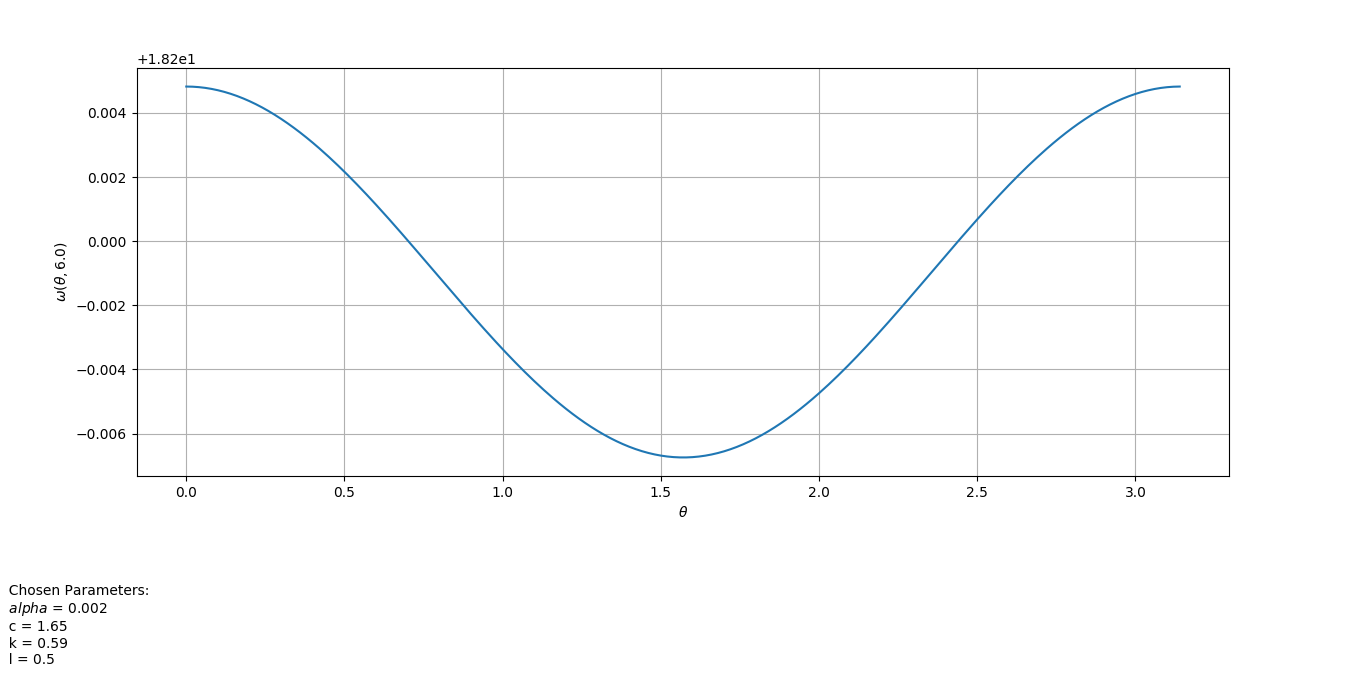
\includegraphics[width=\textwidth,height=\textheight,keepaspectratio]{kir/var_1_t_6.png}                 
	\centering\caption{ График температуры от времени t=6с при $\psi_1(\theta)$}
	\label{grapics1}                           
\end{figure}               

\begin{figure}[H]
    \centering                             
	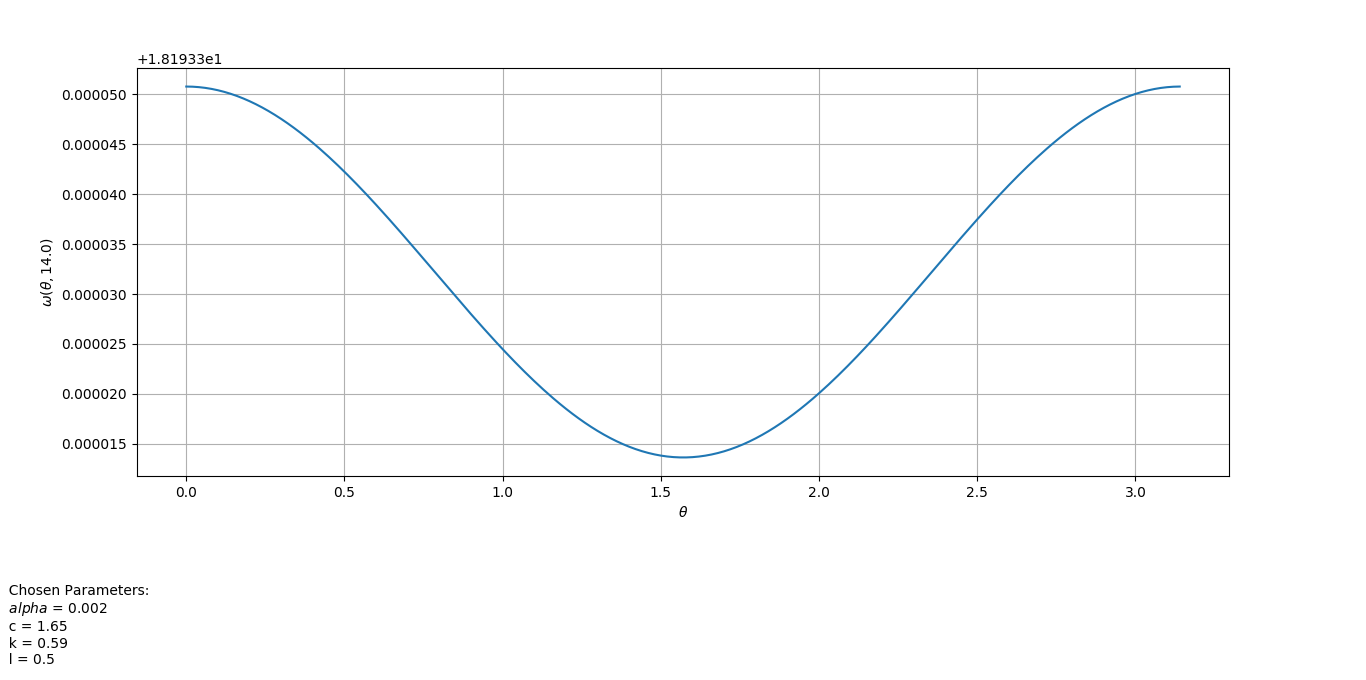
\includegraphics[width=\textwidth,height=\textheight,keepaspectratio]{kir/var_1_t_14.png}                 
	\caption{ График температуры от времени t=14с при $\psi_1(\theta)$}
	\label{grapics2}                           
\end{figure}                                  

\begin{figure}[H]
    \centering                             
	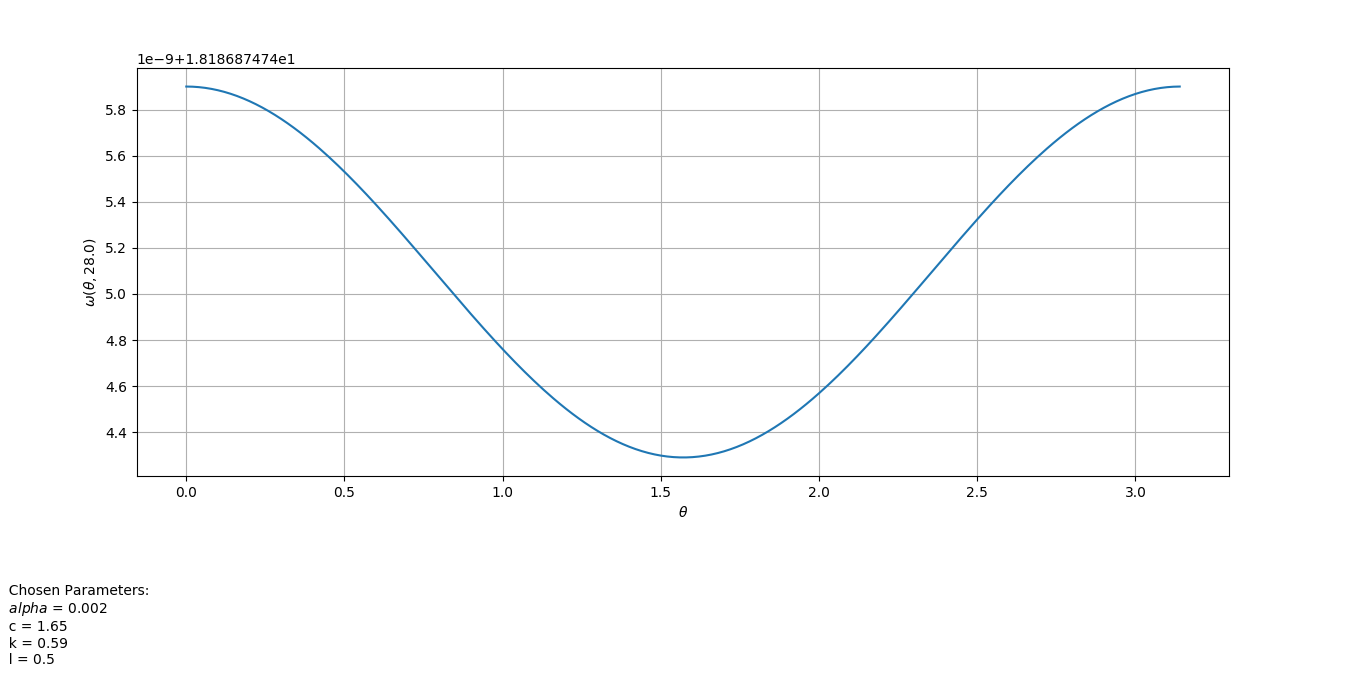
\includegraphics[width=\textwidth,height=\textheight,keepaspectratio]{kir/var_1_t_28.png}                 
	\caption{ График температуры от времени t=28с при $\psi_1(\theta)$}
	\label{grapics3}                           
\end{figure}              
\begin{figure}[H]
    \centering                             
	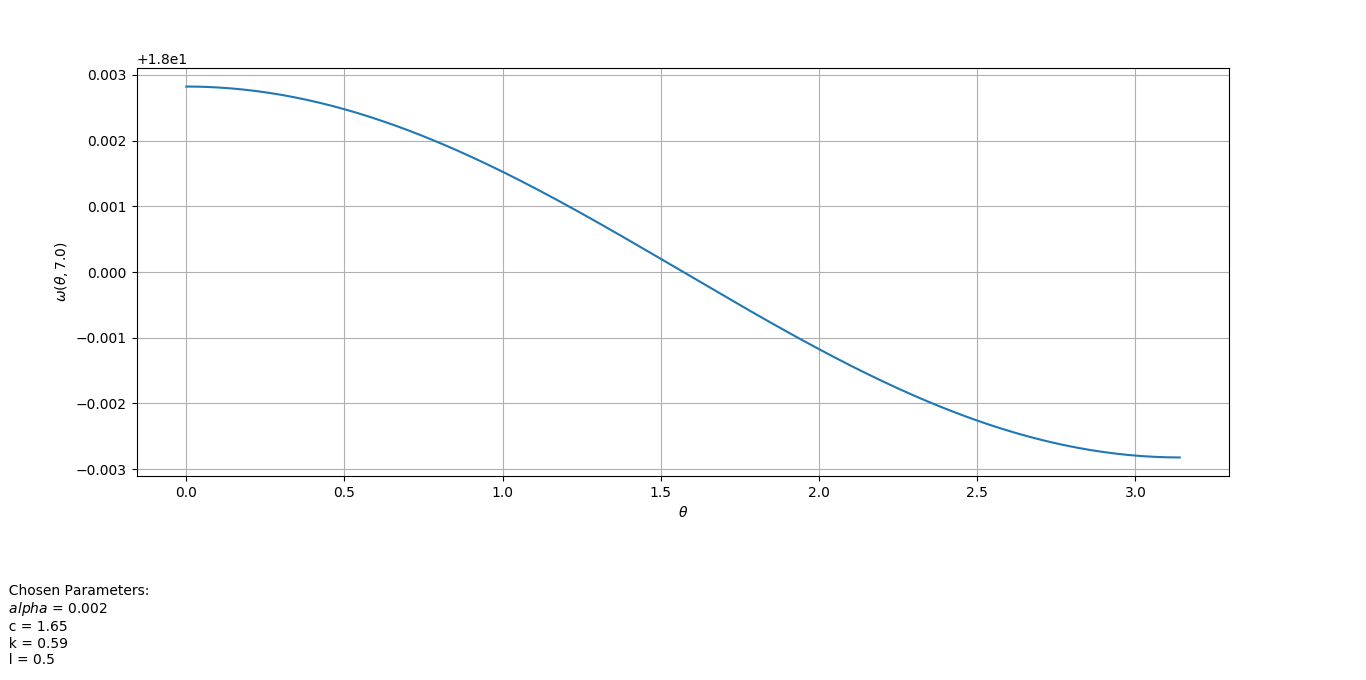
\includegraphics[width=\textwidth,height=\textheight,keepaspectratio]{pos/var_2_t_7.png}                 
	\caption{ График температуры от времени t=7с при $\psi_2(\theta)$}
	\label{grapics4}                           
\end{figure}               

\begin{figure}[H]
    \centering                             
	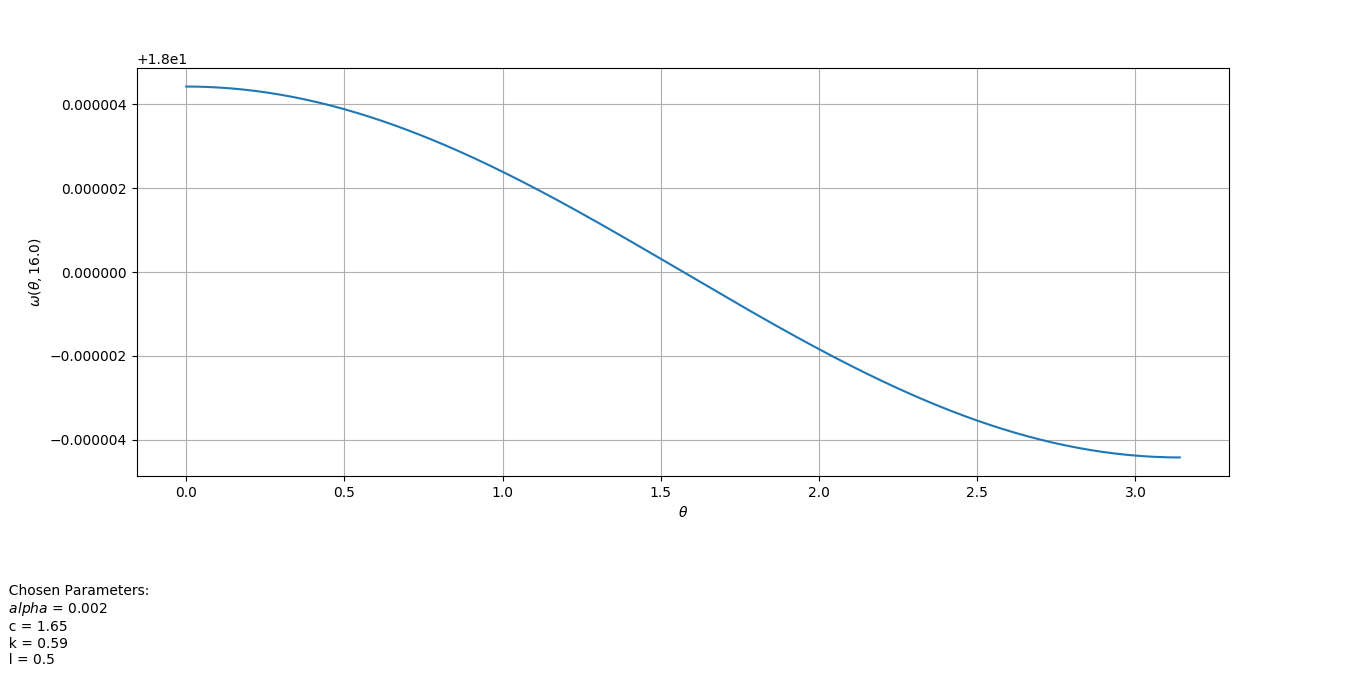
\includegraphics[width=\textwidth,height=\textheight,keepaspectratio]{pos/var_2_t_16.png}                 
	\caption{ График температуры от времени t=16с при $\psi_2(\theta)$}
	\label{grapics5}                           
\end{figure}                                  

\begin{figure}[H]
    \centering                             
	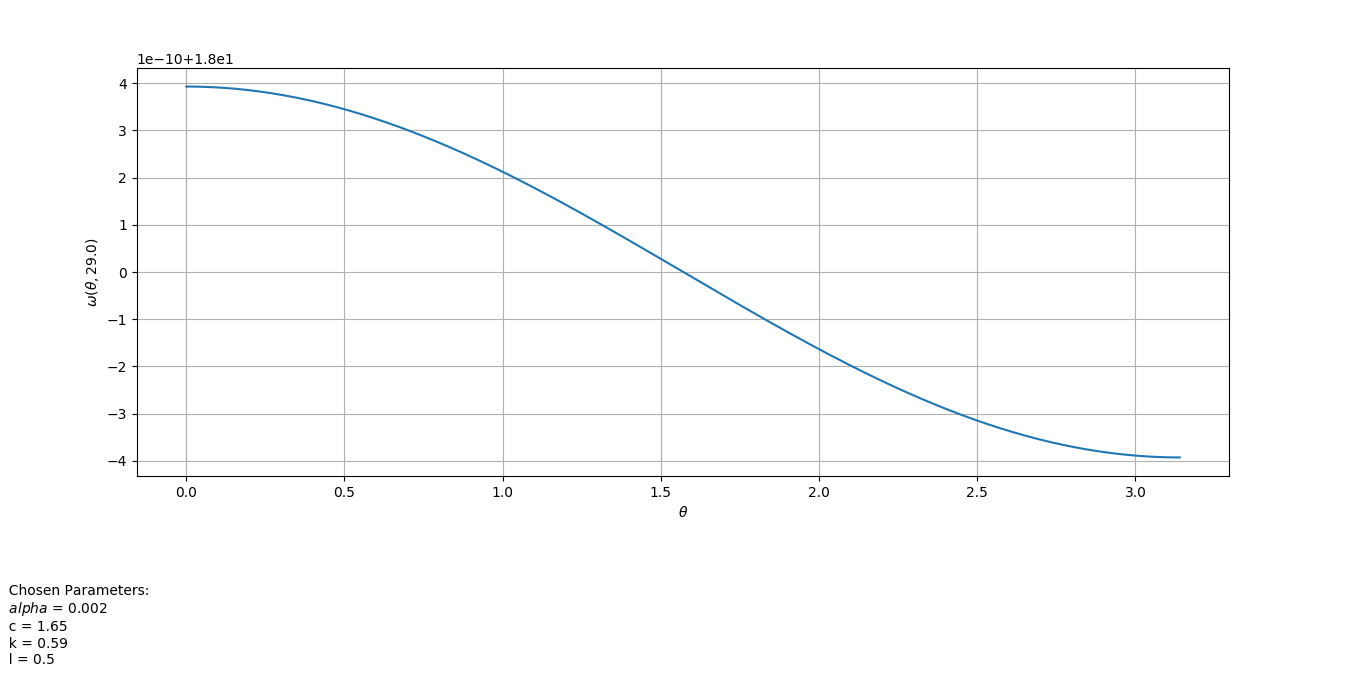
\includegraphics[width=\textwidth,height=\textheight,keepaspectratio]{pos/var_2_t_29.png}                 
	\caption{ График температуры от времени t=29с при $\psi_2(\theta)$}
	\label{grapics6}                           
\end{figure}              

На рисунках \ref{grapics7}, \ref{grapics8}, \ref{grapics9} для начального условия $\psi_1(\theta)$ и \ref{grapics10}, \ref{grapics11}, \ref{grapics12} для $\psi_2(\theta)$, представлены выводы программы зависимости теплоты от времени для различной угловой координаты $\theta$.  

\begin{figure}[H]
    \centering                             
	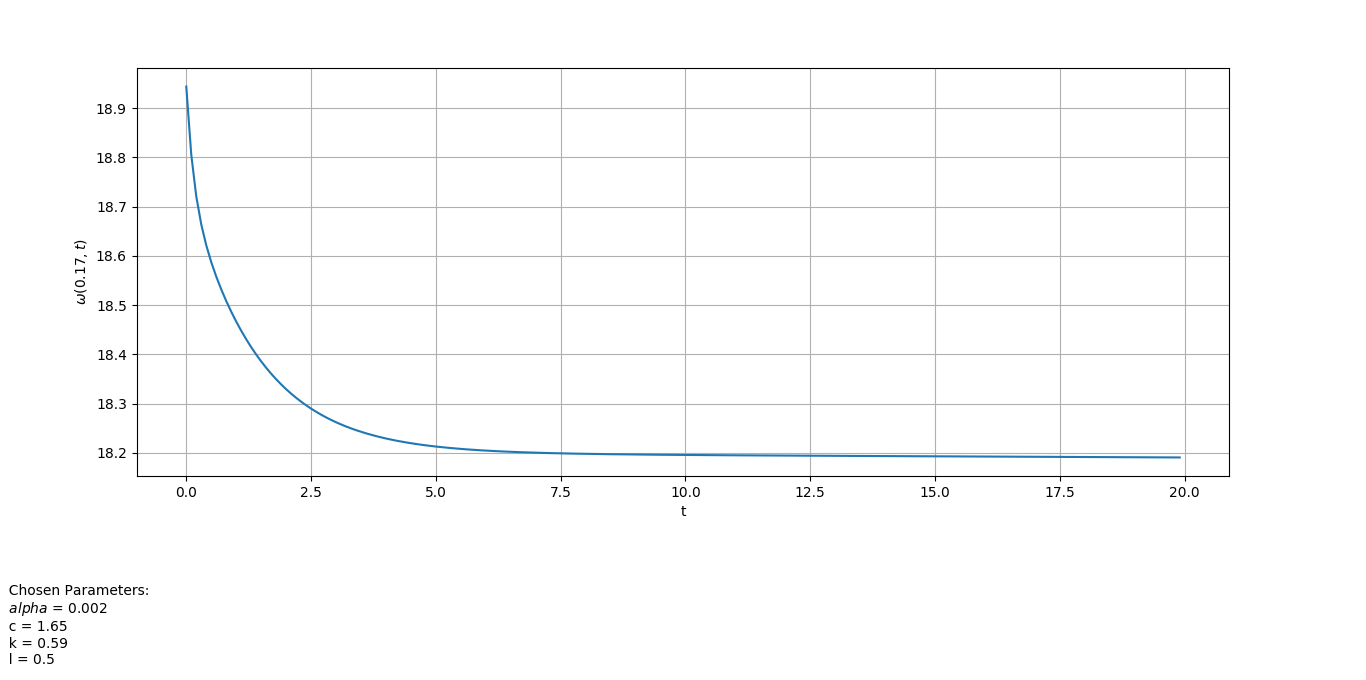
\includegraphics[width=\textwidth,height=\textheight,keepaspectratio]{kir/var_1_z_0t17.png}                 
	\centering\caption{ График температуры от времени $\theta=0.17$ при $\psi_1(\theta)$}
	\label{grapics7}                           
\end{figure}               

\begin{figure}[H]
    \centering                             
	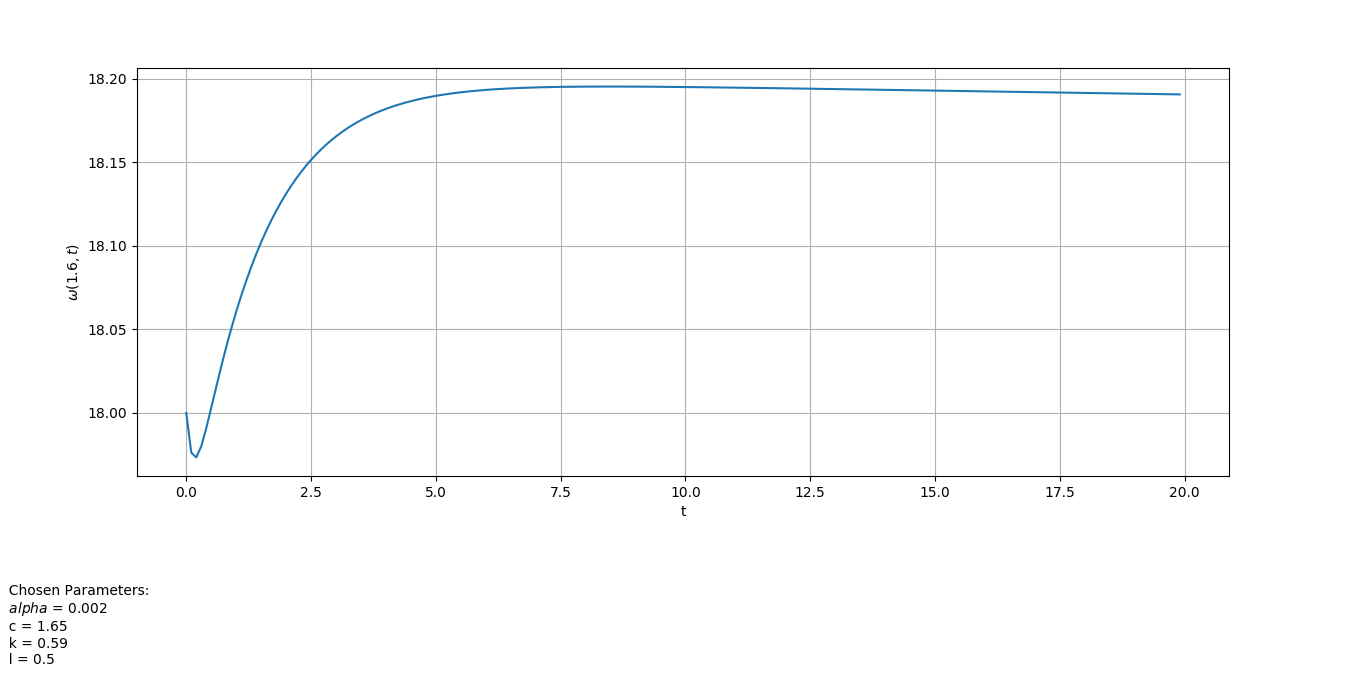
\includegraphics[width=\textwidth,height=\textheight,keepaspectratio]{kir/var_1_z_1t6.png}                 
	\caption{ График температуры от времени $\theta=1.6$ при $\psi_1(\theta)$}
	\label{grapics8}                           
\end{figure}                                  

\begin{figure}[H]
    \centering                             
	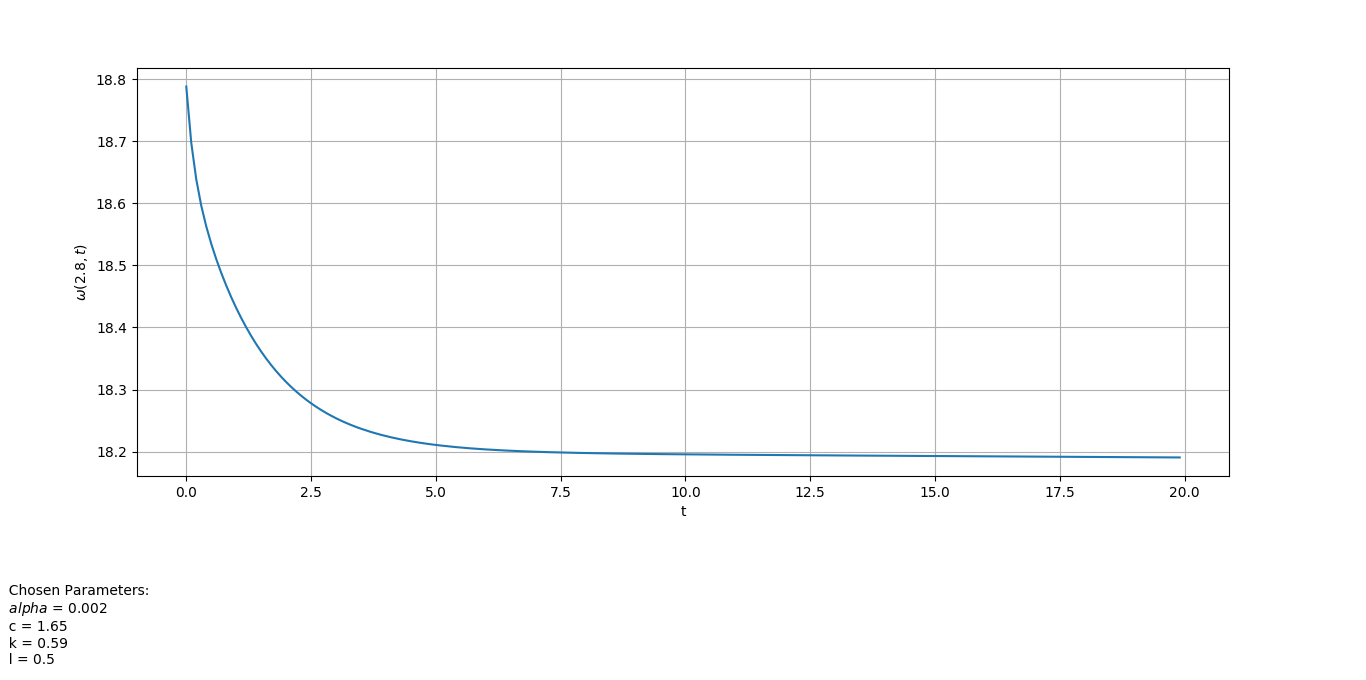
\includegraphics[width=\textwidth,height=\textheight,keepaspectratio]{kir/var_1_z_2t8.png}                 
	\caption{ График температуры от времени $\theta=2.8$ при $\psi_1(\theta)$}
	\label{grapics9}                           
\end{figure}              
\begin{figure}[H]
    \centering                             
	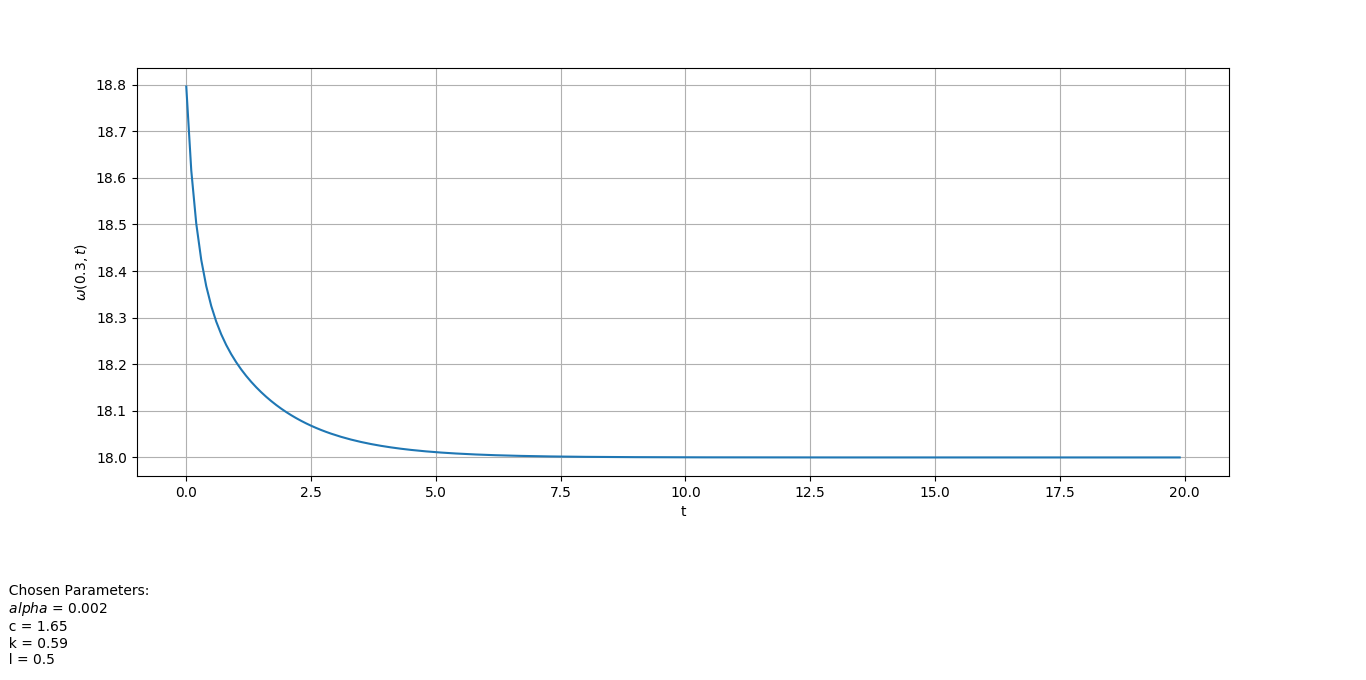
\includegraphics[width=\textwidth,height=\textheight,keepaspectratio]{pos/var_2_z_0t3.png}                 
	\caption{ График температуры от времени $\theta=0.3$ при $\psi_2(\theta)$}
	\label{grapics10}                           
\end{figure}               

\begin{figure}[H]
    \centering                             
	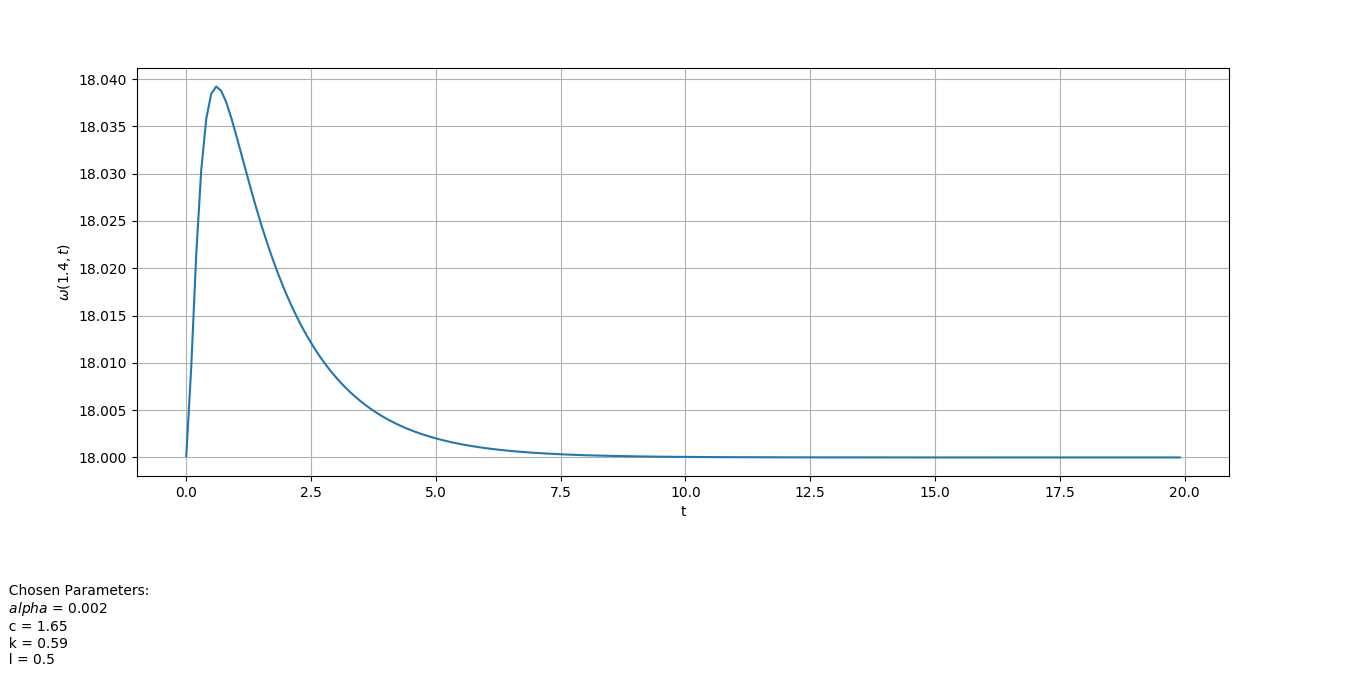
\includegraphics[width=\textwidth,height=\textheight,keepaspectratio]{pos/var_2_z_1t4.png}                 
	\caption{ График температуры от времени $\theta=1.4$ при $\psi_2(\theta)$}
	\label{grapics11}                           
\end{figure}                                  

\begin{figure}[H]
    \centering                             
	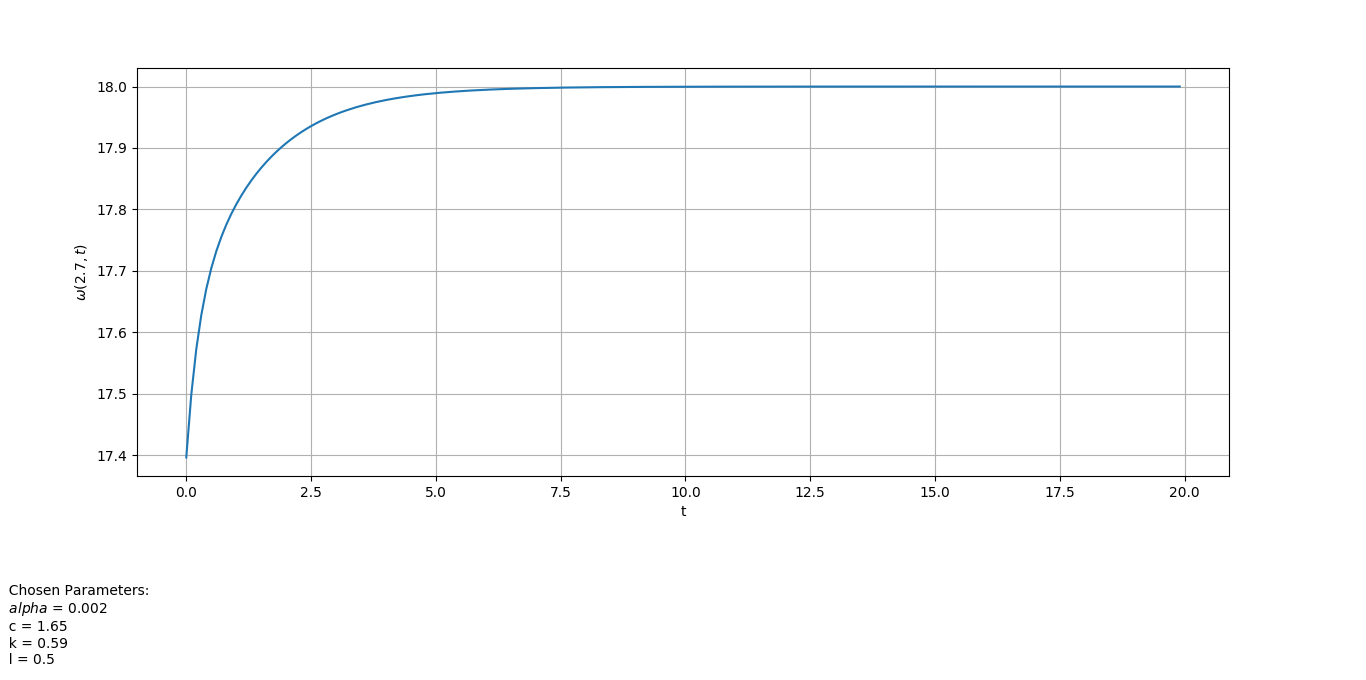
\includegraphics[width=\textwidth,height=\textheight,keepaspectratio]{pos/var_2_z_2t7.png}                 
	\caption{ График температуры от времени $\theta=2.7$ при $\psi_2(\theta)$}
	\label{grapics12}                           
\end{figure}              
                         
                     
    На рисунках с \ref{grapics7} по \ref{grapics12} можно заметить, что в любой точке сферы с увеличением времени
    будет устанавливаться тепловой баланс. А на рисунках с \ref{grapics1} по  \ref{grapics6} видна зависимость распределения температуры на оболочке сферы от начального условия. 
    
}


\newpage
\phantomsection
\addcontentsline{toc}{section}{Заключение}

%------------------------------------------------
% Заключение
%------------------------------------------------

\section*{Заключение}
{
    При выполнении данной работы были изучены аналитические методы решения краевой задачи теплопроводности. Составлена постановка краевой задачи, а также было получено аналитеческое решение в виде конечного ряда Фурье-Лежандра.
    
    
    В ходе работы для решения задачи была написана программа численного моделирования теплового процесса нагревания тонкой оболочки сферы. Данная программа выполняет расчеты темпиратуры с заданными параметрами и позволяет провести анализ погрешности решения для функции начального условия.
     
     
     Анализ полученных результатов показал, что была достигнута достаточно высокая точность решения, при относительно низкой вычислительной сложности.
     Что является хорошим результатом выполненной работы. 
    
}

\newpage
\phantomsection
\addcontentsline{toc}{section}{Список литературы}

%------------------------------------------------
% Список литературы
%------------------------------------------------

\section*{Список литературы}
{
	\begin{enumerate}
	\item \textbf{Дегтярев А.А.} Примеры построения и исследования разностных схем. – Электронное учебное пособие [Электронный ресурс]  / А.А Дегтярев, 2011. - 54с.\label{src1}
    \item \textbf{Тихонов А.Н., Самарский А.А}. Уравнения математической физики(5-е изд.) [Текст]
    / Тихонов А.Н., Самарский А.А. М.: Наука, 1977. - 742 с.\label{src2}
    	\item {Numpy and Scipy Documentation [Электронный ресурс]: Официальный сайт документации библиотек Numpy и Scipy. - URL: https://docs.scipy.org/doc/}\label{src3}
    	\item {MpMath Documentation [Электронный ресурс]: Официальный сайт документации библиотеки MpMath. - URL: http://mpmath.org/doc/current/}\label{src4}
	\end{enumerate}
}

%------------------------------------------------
% Приложения. Коды программ и.т.д.
%------------------------------------------------
\titleformat*{\section}{\large\bfseries\centering}

\newpage
\phantomsection
\addcontentsline{toc}{section}{Приложение А Полиномы Лежандра}
\section*{Приложение А}
{	
	\begin{center}
	\textbf{Полиномы Лежандра}
	\end{center}
     
    Полином Лежандра[\ref{src2}] — многочлен, который в наименьшей степени отклоняется от нуля в смысле среднего квадратического.
    
    Рекуррентная формула для вычисления $n$-го многочлена:
    \begin{equation}
    \left\{
    \begin{split}
    P_{0}(x)    &= 1; \\
    P_{1}(x)    &= x; \\
    P_{n+1}(x)  &= \dfrac{2n + 1}{n+1}xP_{n}(x) - \dfrac{n}{n+1}P_{n-1}(x). 
    \end{split}
    \right.
    \end{equation}    
    
    Первые многочлены Лежандра:
    \begin{align*}
     &P_0(x) = 1; \\
     &P_1(x) = x; \\
     &P_2(x)=\frac{1}{2}(3x^2-1); \\
     &P_3(x)=\frac{1}{2}(5x^3-3x); \\
     &P_4(x)=\frac{1}{8}(35x^4-30x^2+3); \\
     &P_5(x)=\frac{1}{8}(63x^5-70x^3+15x).
    \end{align*}
}

\newpage
\phantomsection
\addcontentsline{toc}{section}{Приложение Б Код программы}
\section*{Приложение Б}
{
	\begin{center}
	\textbf{Код программы}
	\end{center}
	\lstinputlisting[language=Python,mathescape=true]{./src/umf.py}
}

\newpage
\phantomsection
\addcontentsline{toc}{section}{Приложение В Метод квадратур Гаусса-Лежандра}
\section*{Приложение В}
{
\begin{center}
	\textbf{Метод квадратур Гаусса-Лежандра}
	\end{center}
	
	Метод квадратур Гаусса-Лежандра - метод численного интегрирования, в основе которого лежит метод квадратур Гаусса.
	Особенностью метода является то, что он позволяет повысить алгебраический порядок точности, без увеличения числа 
	используемых значений подынтегральной функции. 
	Тем самым может быть достигнута максимальная точность для выбранного числа узлов интегрирования.
	Численное интегрирование методом Гаусса вычисляется по формуле:
	\begin{equation}
	    I \approx \sum_{i=1}^{n}{\omega_i f(x_i)},
	\end{equation}
	где $x_i$ - узлы интегрирования, а $\omega_i$ - ненулевая константа, называемая ``вес квадратуры``.
	
	Для вычисления методом Гаусса-Лежандра веса вычисляются по следующей формуле:
	\begin{equation}
	    \omega_i = \dfrac{2}{(1-x^{2}_{i})\left[ P'_n(x_i) \right]^2},
	\end{equation}
	где $P'_n(x_i)$ - первая производная $n$-го полинома Лежандра, который описан в приложении А, 
	$x_i$ - корни полинома Лежандра.
	
	Для нахождения производной многочлена Лежандра $n$-го порядка используется следующая рекуррентная формула:
	\begin{equation}
	    P'_n(x) = \dfrac{n}{x^2 - 1}\left(xP_{n}(x) - P_{n-1}(x) \right)
	\end{equation}
	
    Многочлены Лежандра, в основном, не имеют аналитического решения и находятся через аппроксимирующие численные методы для нахождения корней.
    На практике чаще всего используется метод касательной (Модификация метода Ньютона), который вычисляется по формуле:
     \begin{equation}
         x_{i+1} = x_i - \dfrac{P_n(x_i)}{P_n'(x_i)}
     \end{equation}
     Для начального приближения $i$-го корня полинома Лежандра степени $n$ берется
     $$x_0 = \text{cos}\left(\pi\dfrac{i - \dfrac{1}{4}}{n + \dfrac{1}{2}}\right)$$
     
     Конечная формула для численного интегрирования:
     \begin{equation}
     \int\limits_{a}^{b}{f(x)} dx \approx \dfrac{b-a}{2}\sum_{i=1}^{n}{\omega_{i}f\left(\dfrac{b-a}{2}x_{i} + \dfrac{a+b}{2}\right)}
     \end{equation}
}
\end{document}
